\chapter{Introduction}
In the dynamic digital age, rapid and easy access to an immense repository of information has revolutionised the way knowledge is sought and consumed. Retrieval pipelines are the technological backbone behind search engines and recommendation systems, providing guidance through this vast information landscape. These pipelines are indispensable in people's daily lives, making them a vital component of a digital existence.

The performance of retrieval pipelines is inextricably linked to the myriad of ways users formulate queries. Queries can exhibit various variations encompassing nuances in wording, syntax, and structure. Despite these distinctions, the ultimate goal remains constant – to satisfy the user's underlying information requirement.

Recognising how these variations exert their influence on the performance of retrieval pipelines is of paramount importance in the ongoing investigation of ensuring these systems remain in harmony with the ever-evolving needs of their users. These variations can introduce substantial challenges to the search and recommendation process. Understanding and addressing them is pivotal to maintaining the reliability and effectiveness of these systems in serving the ever-diversifying needs of a global population that relies on them as indispensable tools in navigating the information-rich digital landscape. It is this constant adaptation and evolution of retrieval pipelines that guarantees they continue to be the reliable guides we depend on in our digital quests for knowledge and information.

\section{Objectives and Scope}
This thesis embarks on a comprehensive exploration of the robustness and generalisability of findings from an original study conducted in information retrieval. The study in question, authored by Gustavo Penha, Arthur Câmara, and Claudia Hauf \cite{penha2022}, is titled "Evaluating the Robustness of Retrieval Pipelines with Query Variation Generators." Hereafter referred to as the "original study," this research has contributed invaluable insights into the performance of retrieval pipelines when subjected to variations in search queries. In particular, it has shed light on the limitations of these systems and proposed potential strategies for their improvement.

This study is motivated by the pursuit of a deeper understanding of the behaviour of retrieval systems and the broader implications of the original study's findings, mainly when applied to different datasets and conditions. To accomplish this, two fundamental research questions guide the overarching themes of this investigation:

\subsubsection{Research Question 1 (RQ1):}
To what extent can the findings and observations from the original study be successfully replicated using the same datasets, models, and methodologies?

\subsubsection{Research Question 2 (RQ2):}
How do the conclusions drawn from the original study generalise when applied to additional datasets, and what insights can be gained from this broader perspective?

\subsection{Research Question 1: Reproduction}
Research Question 1 dives deeply into the critical aspect of assessing the reproducibility of findings and observations from the original study, aiming to provide a comprehensive understanding of the robustness and reliability of the original research. This is a pivotal step in scientific inquiry as it not only validates the credibility of the initial findings but also paves the way for further development and refinement of knowledge in the field.

To address this research question, the study meticulously recreates the experimental conditions, utilising the same datasets, models, and methodologies employed in the original research. By doing so, it seeks to answer the fundamental question of to what extent the original study's results can be successfully replicated. This replication process is essential as it offers a crucial litmus test for the validity and trustworthiness of the original study's outcomes.

Moreover, the investigation of reproducibility is not just about confirming the original findings; it also serves as a means to uncover the intricacies and subtleties of the observed phenomena. By repeating the experiments under identical conditions, researchers gain a deeper insight into the inherent stability and robustness of these phenomena. This, in turn, contributes significantly to the development of more resilient retrieval pipelines, providing a solid foundation upon which future advancements can be built.

The objectives of Research Question 1 can be further delineated into two primary goals. First and foremost, it seeks to recreate the critical findings of the original study using the same datasets, models, and methodologies. This replication process is integral in determining the reliability and stability of the original observations. By successfully reproducing the results, it reinforces the credibility of the initial study's findings, adding weight to its scientific merit.

Secondly, Research Question 1 endeavours to identify any potential discrepancies or variations that may arise during the reproduction process. These deviations, if they occur, are not to be dismissed but rather subjected to thorough scrutiny. These factors can encompass a myriad of variables, including differences in the characteristics of the datasets used, variations in model behaviour, or subtle nuances in the methodology employed. Understanding these variations is essential as it not only highlights potential limitations of the original study but also provides valuable insights into the broader context of the research, which can aid in refining future studies and enhancing the overall understanding of the field.

\subsection{Research Question 2: Expansion}
The second research question studies the generalisability of the original study's conclusions when applied to additional datasets. The original study, while providing valuable insights, was confined to specific datasets, and this limited scope raises essential questions about the transferability of its findings to a broader context. In essence, we aim to ascertain how well the conclusions drawn from the original study extend to a more diverse spectrum of datasets, and this broader perspective is essential for a comprehensive understanding of the phenomena under investigation.

The objective of Research Question 2 is to systematically explore how the insights and conclusions of the original study stand up when exposed to a wide array of datasets beyond those initially considered. This involves the rigorous application of the same methodologies, models, and analytical tools used in the original study to the additional dataset. By subjecting these datasets to the same analytical lens, this research strives to uncover nuances and insights that may emerge in different dataset contexts. This process not only enhances the comprehension of the generalisability of the original study's findings but also contributes to a more robust understanding of retrieval pipeline behaviour across many scenarios.

By investigating the generalisability of the original study's conclusions in diverse dataset contexts, a more comprehensive and nuanced perspective on the studied phenomena is gained. This approach allows for identifying overarching trends and patterns that may transcend the specific dataset used in the original research, thus expanding our knowledge and refining the conclusions drawn from the study. 

\subsection{Scope}
This research project is focused on investigating the impact of query variations on the effectiveness of retrieval pipelines in the context of large language models, specifically examining the DL-TYPO dataset. The following aspects fall within the project scope:

\subsubsection{In Scope:}
\begin{itemize}
    \item Query Variation Categories: The project will explore and evaluate the impact of query variations within categories such as misspellings, paraphrasing, naturality, and ordering. These categories align with the variations previously studied in the original research.
    \item Existing Models and Methods: The research will employ existing models and query variation methods utilised in the original study. This includes RandomOrderSwap, NeighbCharSwap, QWERTYCharSub, RandomCharSub, RemoveStopWords, T5DescToTitle, WordEmbedSynSwap, T5QQP, BackTranslation, and WordNetSynSwap.
    \item Evaluation Metrics: The evaluation will use standard information retrieval metrics such as nDCG@10 to assess the effectiveness of retrieval pipelines when confronted with query variations.
    \item Datasets: The project will extend to focus on the DL-TYPO dataset, which contains queries with typos. Additionally, it will encompass the ANTIQUE and TREC-DL-2019 datasets used in the original study, providing a basis for comparison and validation.
\end{itemize}

\subsubsection{Out of Scope:}
\begin{itemize}
    \item New Models or Generator Techniques: The project will not involve the development or implementation of new models or generator techniques for query variations. It will rely on the existing methods established in the original research.
    \item Online Evaluation: Online evaluation methods, which require real-time user interactions and feedback, are not within the scope of this project. The research will primarily focus on offline evaluation metrics.
    \item Query Variation Categories: The project will not investigate variation types that alter semantics (e.g., changing the meaning of the query). It primarily concerns variations that do not significantly change the underlying user intent.
\end{itemize}

\section{Project Timeline}
This section examines how the actual timeline of the thesis project aligned with the projected timeline outlined in the initial proposal, graphically represented in \fig{fig:gantt}. It is essential to highlight that while the project plan serves as a structured guide, unforeseen challenges and adjustments often occur during the execution of any research endeavour. In this case, deviations from the initially projected timeline impacted the project's progress.

\begin{figure}[h]
    \centering
    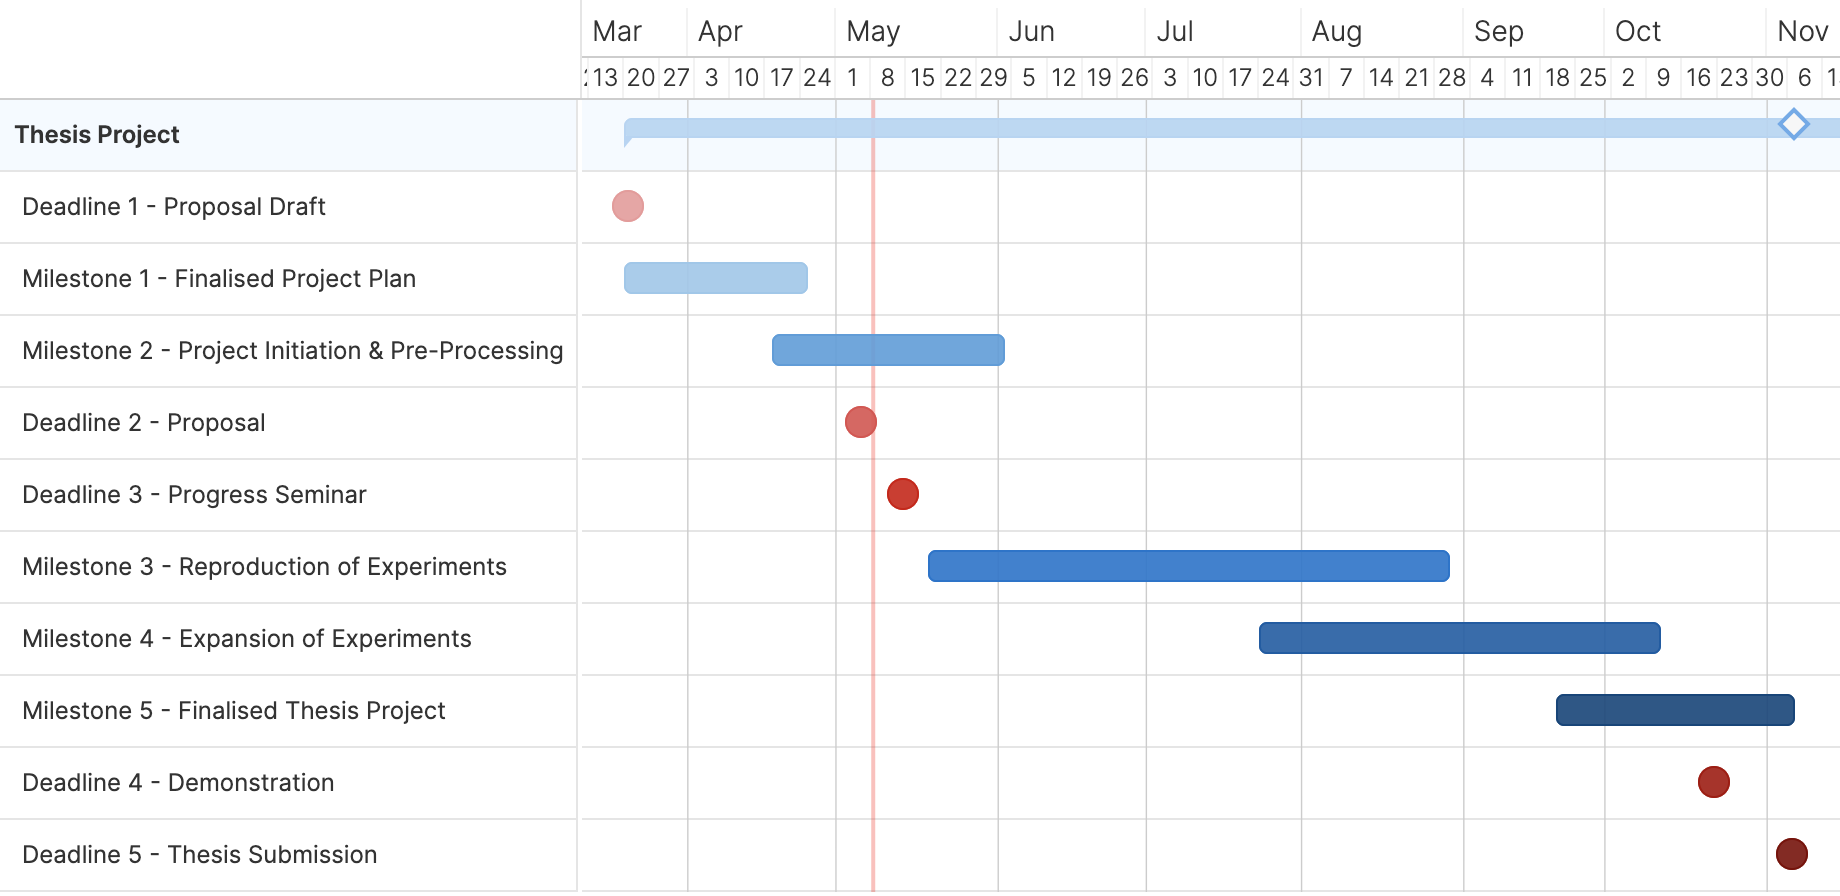
\includegraphics[width=\textwidth]{1Introduction/GanttChart.png}
    \caption{Gantt chart representing predicted project timeline.}
    \label{fig:gantt}
\end{figure}

\subsubsection{Project Initiation \& Pre-Processing}
The initiation phase of the project, Milestone 2, which was intended to focus primarily on pre-processing datasets, was instead utilised to set up the codebase and establish the computational environment. This deviation from the original plan was driven by the necessity to create a foundation for the subsequent phases of the project. Specifically, a Google Colab environment with GPU capabilities had to be set up to accommodate the resource-intensive tasks involved in the experiment reproduction and expansion. This process introduced some delays in the timeline, as configuring the environment and ensuring compatibility with the required tools and libraries proved more time-consuming than initially anticipated.

\subsubsection{Impact on the Expansion of Experiments}
Due to the delays experienced in the initial phase, the commencement of the "Reproduction of Experiments" milestone was postponed. Consequently, the time allocated for expansion of the experiments was shorter than initially projected. There were some limitations in the extent of extra data analysis compared to the original study. However, it is essential to note that all fundamental aspects of the project, including the implementation of ranking models and query generation, were diligently pursued.

Throughout the project, flexibility and adaptability were demonstrated in response to the challenges encountered. This flexibility allowed for the management of the project's evolving timeline and the delivery of meaningful results. The adjustment in the schedule ensured that the project continued to meet its primary objectives, although some stages took longer than initially planned.

\section{Thesis Structure}
The thesis is organised into several essential chapters, each dedicated to specific aspects of the research inquiry. It commences with the introductory chapter (Chapter 1), establishing the foundation by presenting two pivotal research questions and outlining the objectives. This chapter also offers an overview of the thesis's timeline and structure.

Following the introduction, Chapter 2 delves into the necessary background information to comprehensively understand information retrieval, natural language processing, ranking models, and evaluation metrics. This chapter lays the theoretical groundwork upon which subsequent analyses are constructed.

Chapter 3 explores the landscape of related work, focusing on previous research on large language models, enhancements in retrieval pipelines, evaluation metrics, and query variation techniques. This contextualisation provides insights into the existing body of knowledge and underscores the significance of the present research.

In Chapter 4, the methodology utilised for conducting experiments is elaborated upon. This includes the description of datasets used, ranking models, training processes, query generators, assessment of query generator quality, and the application of evaluation metrics. A thorough understanding of this methodology is crucial for comprehending the subsequent empirical findings.

Chapter 5 presents the results and discussions arising from the empirical investigations, divided into three sections, each corresponding to generation quality and one of the research questions posed in the introduction.

The final chapter, Chapter 6, serves as the conclusion and culmination of the thesis. It summarises the research's primary findings and conclusions, addressing the research questions. Furthermore, it reflects on future research avenues, identifying areas in information retrieval and query variation analysis that warrant further exploration.
